\documentclass[border=10pt]{standalone}
\usepackage{tikz}
\usetikzlibrary{arrows.meta, positioning, fit, backgrounds}

\definecolor{convblue}{HTML}{0077B6}
\definecolor{agentamber}{HTML}{E8B517}
\definecolor{passgreen}{HTML}{2D6A4F}
\definecolor{txtgray}{HTML}{4A4A4A}

\begin{document}
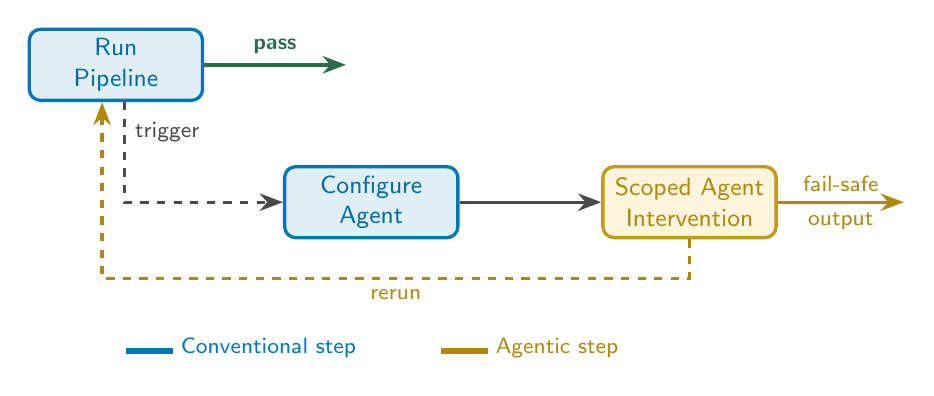
\begin{tikzpicture}[
    >=Stealth,
    font=\sffamily\small,
    text=txtgray,
    node distance=1.4cm and 1.8cm,
    convbox/.style={
        draw=convblue, fill=convblue!12, rounded corners=4pt,
        minimum height=0.9cm, minimum width=2.2cm, align=center,
        font=\sffamily\small, text=convblue!90!black,
        line width=1.2pt,
    },
    agentbox/.style={
        draw=agentamber!85!black, fill=agentamber!15, rounded corners=4pt,
        minimum height=0.9cm, minimum width=2.2cm, align=center,
        font=\sffamily\small, text=agentamber!75!black,
        line width=1.2pt,
    },
    arr/.style={->, very thick, color=txtgray},
]

% Run Pipeline at top level
\node[convbox] (pipeline) {Run\\Pipeline};

% Pass arrow — default/happy path going right
\draw[arr, passgreen] (pipeline.east) -- ++(1.8,0) node[above, midway, font=\sffamily\footnotesize\bfseries, passgreen] {pass};

% Trigger path — slightly below Run Pipeline
\node[convbox, below right=0.8cm and 1.0cm of pipeline] (catch) {Configure\\Agent};
\node[agentbox, right=of catch] (intervene) {Scoped Agent\\Intervention};

% Trigger arrow from pipeline down to catch — exits right of center
\draw[arr, dashed] ([xshift=3pt]pipeline.south) |- (catch)
    node[right, pos=0.15, font=\sffamily\footnotesize, txtgray] {trigger};
\draw[arr] (catch) -- (intervene);

% Rerun — loop back from intervene, enters pipeline at left side
\draw[arr, agentamber!75!black, dashed]
    (intervene.south) -- ++(0,-0.5)
    -| node[below, near start, font=\sffamily\footnotesize, agentamber!75!black] {rerun}
    ([xshift=-5pt]pipeline.south);

% Fail-safe output — arrow going right from intervene
\draw[arr, agentamber!75!black] (intervene.east) -- ++(1.6,0)
    node[above, midway, font=\sffamily\footnotesize, agentamber!75!black] {fail-safe}
    node[below, midway, font=\sffamily\footnotesize, agentamber!75!black] {output};

% Legend
\node[convblue, font=\sffamily\footnotesize, anchor=west] at (0,-3.6)
    {\rule{0.6cm}{2pt}\ Conventional step};
\node[agentamber!75!black, font=\sffamily\footnotesize, anchor=west] at (4.0,-3.6)
    {\rule{0.6cm}{2pt}\ Agentic step};

\end{tikzpicture}
\end{document}
